\vspace{-3mm}
\section{Materialverhalten}{}
    \subsection{Festigkeitshypothesen}
        \subsubsection{Fliessbedingung/Fliessfunktion $\Phi(\sigma)$}
            Fliessbedingung: $\Phi(\sigma)<0$ (elastisch), $\Phi(\sigma)=0$ (plastisch)
            \begin{center}
            \vspace{-2mm}
                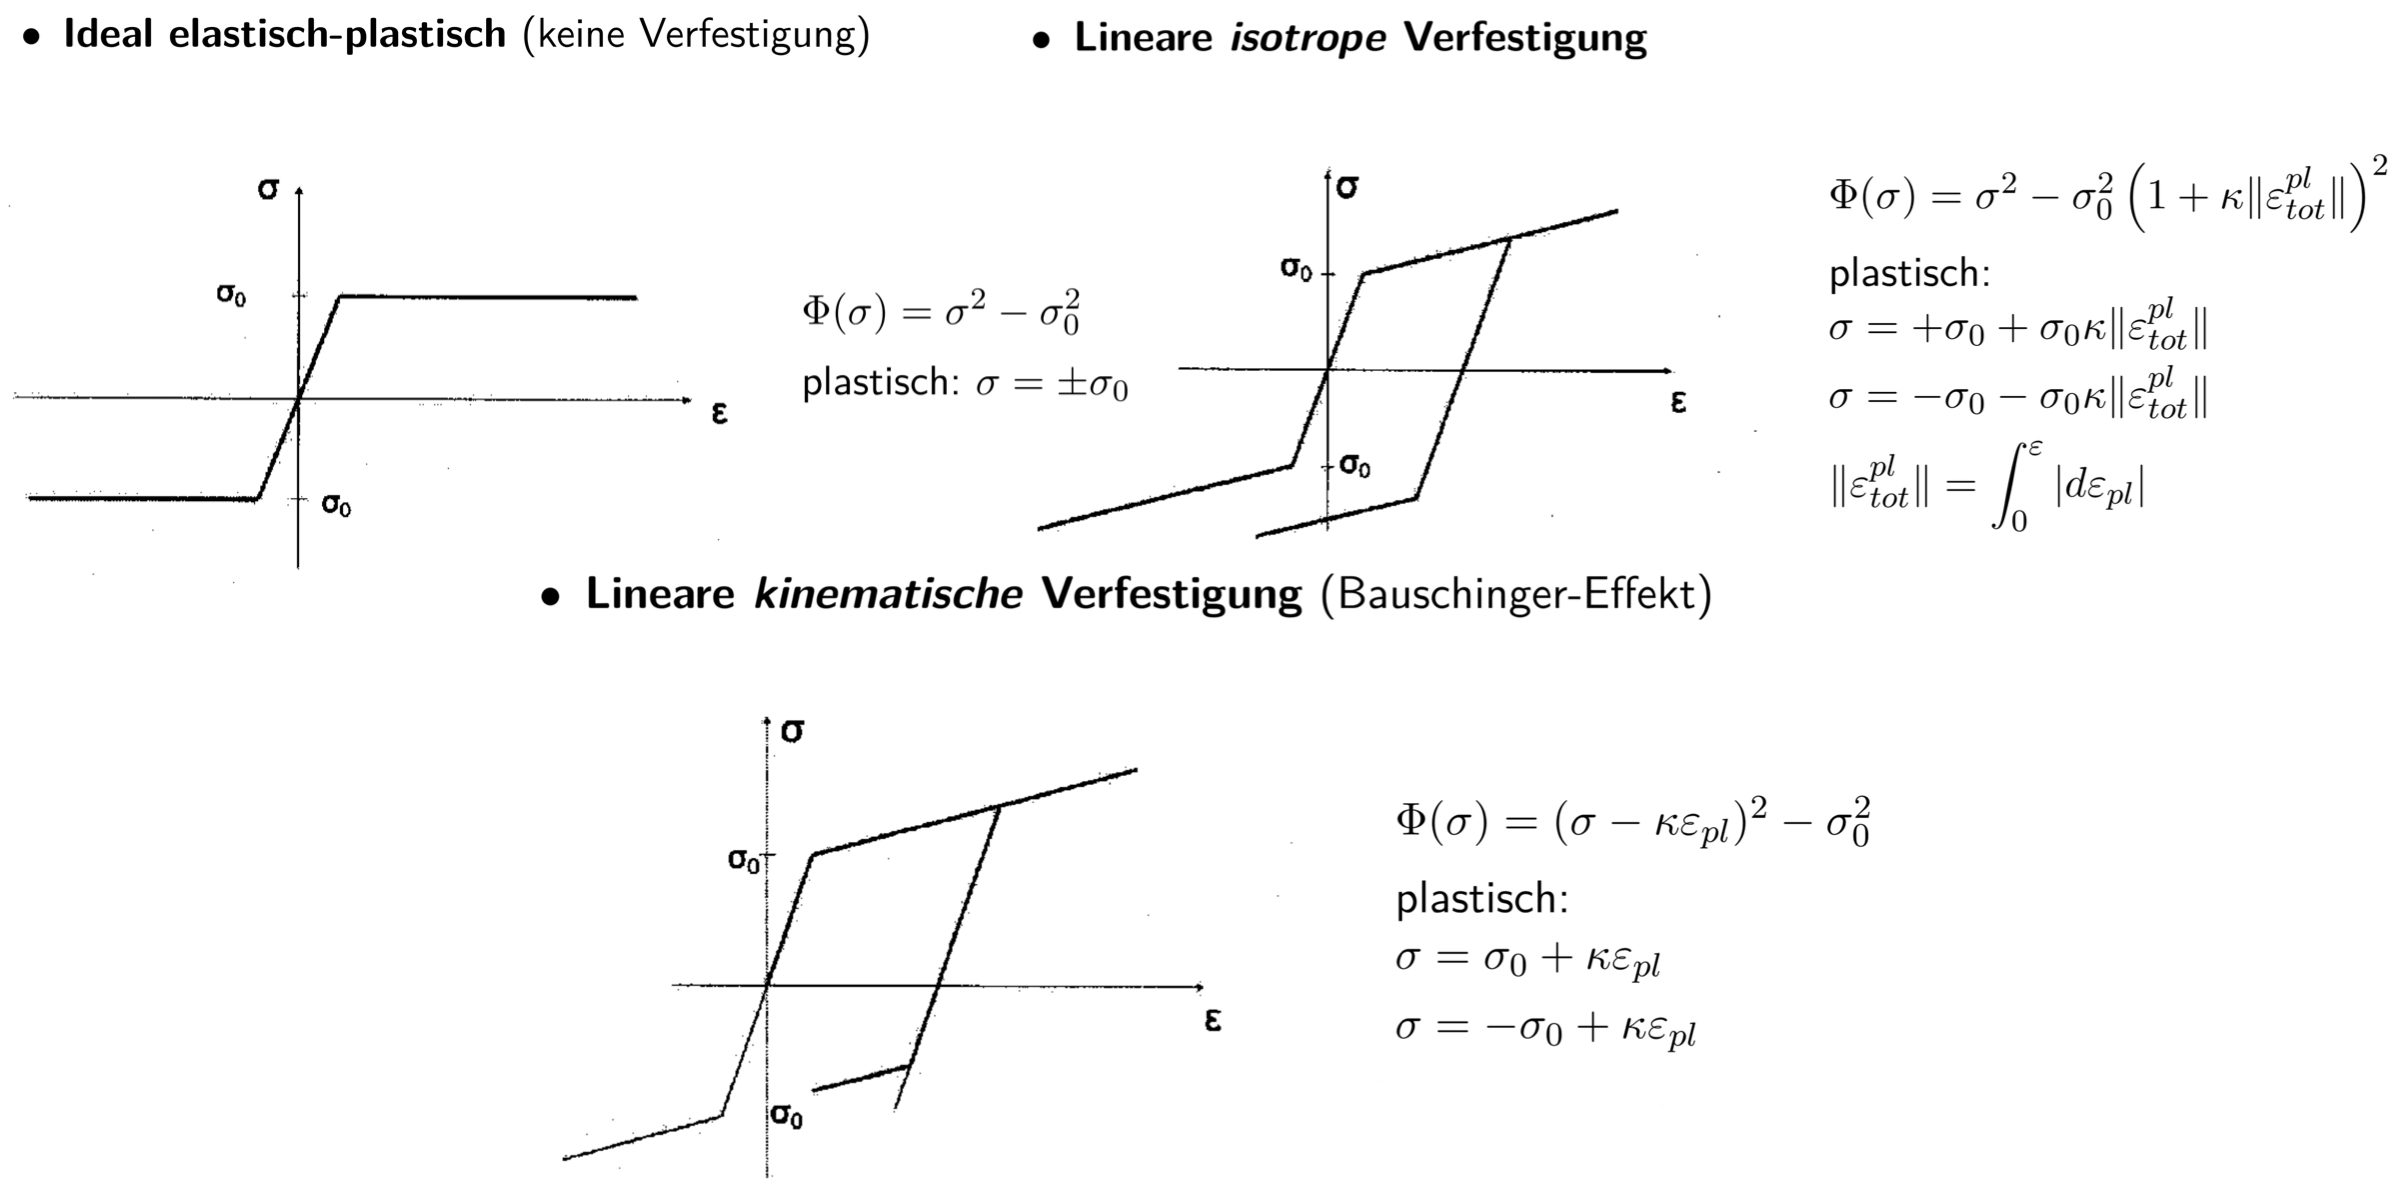
\includegraphics[width=0.9\linewidth,]{04/fliessbedingungen.jpeg}
            \end{center}
            
        \subsubsection{von Mieses'sche Vergleichsspannung}
            \[\Phi_{\textrm{v.Mises}}= \sigma_1^2+\sigma_2^2+\sigma_3^2-\sigma_1\sigma_2-\sigma_1\sigma_3-\sigma_2\sigma_3 -\sigma_0^2\quad(=0)\]
            \[\Leftrightarrow \sigma_{\textrm{v. Mises}}^{vgl}= \sqrt{\sigma_1^2+\sigma_2^2+\sigma_3^2-\sigma_1\sigma_2-\sigma_1\sigma_3-\sigma_2\sigma_3} \quad\textrm(HS)\]
            Experiment: Fliessen ist unabhängig vom hydrostatischen Spannungszustand.
        \subsubsection{Tresca'sche Vergleichsspannung (maximale Schubspannungshypothese)}
            \textbf{Konservativer} als von Mises'sche Vergleichsspannung (Grenzfläche von Sechseck schneller erreicht als von Ellipse).
            \vspace{-2mm}\[\sigma_{\textrm{Tresca}}^{vgl}=\textrm{max} \left(|\sigma_1-\sigma_2|,|\sigma_2-\sigma_3|,|\sigma_3-\sigma_1| \right) =2\tau_0\]
    \subsection{Statische Belastung}
        
            \subsubsection{Kraft- \& Deformationsgesteurete Belastung:}
            $\frac{\varepsilon_b}{\varepsilon_0}$ \textbf{Deformationsgesteuerte Belastung:} Bspw vorgespannte Schraube oder thermische Spannungen. Hier ist die Begrenzung der auftretenden Spannungen weniger konservativ, da plastische Deformationen zur Reduktion der pseudo-elastischen Spannungen führen. $\sigma$-$\varepsilon$-Diagramm: gr Dehnung führt zu nur kl Spannungserhöhung). Beeinflussen Grenzlast nicht.\\\\ 
            $\frac{\sigma_B}{\sigma_0}$ \textbf{Kraftgesteuerte Belastung:} (Für viele Metalle $\frac{\varepsilon_b}{\varepsilon_0} \gg \frac{\sigma_B}{\sigma_0}$) Beim Überschreiten von $R_{p0.2}$ oft weniger Reserve $\rightarrow$ konservativere Dimensionierung.
        
        \subsubsection{Spannungsverteilung}
            Falls homogen: bei Fliessgrenze wird die ganze Struktur plastifiziert. $\rightarrow$ Versagen %bei Erreichen der Fliessgrenze wird es in der ganzen Struktur zur Plastifizierung kommen. 
              
            Falls linear: es kommt an lokalen Stellen zu Plastifizierungen $\rightarrow$ Versagen erst bei einer grösseren Belastung.\\
            \textbf{Zug:}
            \vspace{-2mm}
            \begin{itemize}
                \item Erste plastifizierung = vollständige Plastifizierung:
            \end{itemize}
            \vspace{-2mm}
            \begin{center}
                $\displaystyle F_{plast} = \sigma_0\ \cdot A$
            \end{center}
            
            %\columnbreak
            \vspace{-4mm}
\vfill\null\columnbreak
            \textbf{Biegung:}
            \vspace{-2mm}
            \begin{itemize}
                \item Erste Plastifizierung:
            \end{itemize}
            \[M_{plast} = \sigma_0\cdot I\cdot\frac{1}{y_{\textrm{max}}} \quad\textrm{(mit bspw $\sigma_0 = R_p$)}\]
            \begin{itemize}
                \item Vollständige Plastifizierung:
            \end{itemize}
            \[M_{versagen} = 2\int_{-b/2}^{b/2}\int_{0}^{h/2}\sigma(y)ydydz \quad\textrm{mit $\sigma(y) = \sigma_0$}\]
            
        \subsubsection{Formfaktoren}
            \textit{Spannungsverteilung homogen:} (Zug ideal plastisch) $f=1$.
            \\\textit{Spannungsverteilung als lineare Funktion:} Fliessgrenze an einem Ort überschritten (1. Plastifizierung) aber grösster Teil des Querschnittes noch elastisch $\rightarrow$ Reserve. (Bsp. Biegung bei elastisch ideal-plastisch)
            \[f=\frac{M_{versagen}}{M_{plastifizierung}}\]
            \begin{center}
                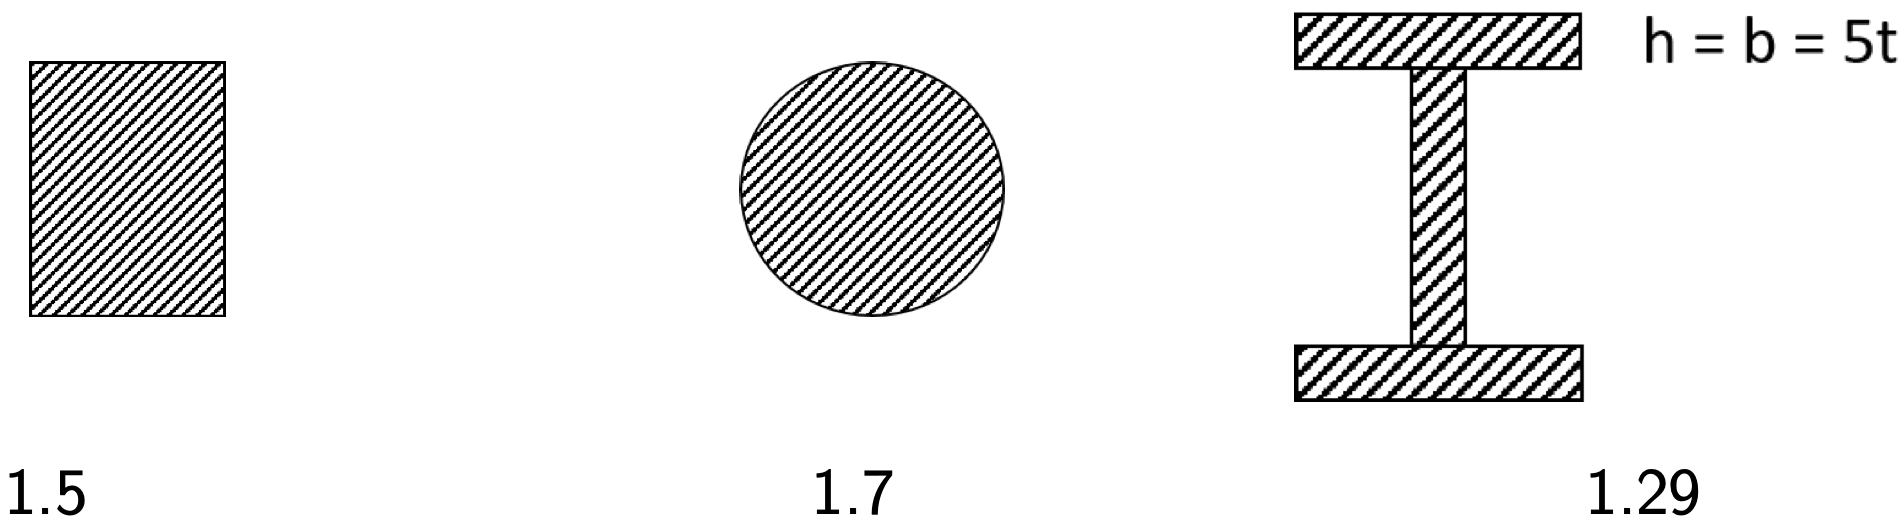
\includegraphics[width=0.6\linewidth]{04/formfaktoren.png}
            \end{center}
    
            